\chapter{Estado de la Cuestión}
\label{cap:estadoDeLaCuestion}

%Citaremos con bibtex, las entradas bibliográficas deben estar en un fichero .bib 

\section{Enfermedad de Alzheimer}
El Alzheimer, una enfermedad neurodegenerativa progresiva y devastadora, afecta a millones de personas en todo el mundo. Se caracteriza por la pérdida gradual de la memoria y otras funciones cognitivas, lo que eventualmente conduce a la incapacidad para llevar a cabo las actividades diarias más básicas. Su curso clínico se divide en varias etapas distintas, cada una con sus propias características y desafíos.
\begin{itemize}
\item Etapa Temprana o Leve:\\
En esta fase inicial, los síntomas pueden pasar desapercibidos o atribuirse a simples descuidos. La persona afectada puede experimentar dificultades para recordar nombres, eventos recientes o encontrar las palabras adecuadas en conversaciones. A pesar de estos desafíos, generalmente conservan la capacidad de realizar tareas cotidianas con cierta independencia. Sin embargo, es posible que comiencen a perder interés en actividades previamente disfrutadas.

\item Etapa Intermedia o Moderada:\\
A medida que la enfermedad progresa, los síntomas se vuelven más evidentes y problemáticos. La pérdida de memoria se vuelve más pronunciada, con dificultades para reconocer a familiares y amigos cercanos. Además, pueden surgir problemas de orientación en tiempo y espacio, lo que puede resultar en desorientación incluso en entornos familiares. Las habilidades de comunicación también se ven afectadas, con dificultades para seguir conversaciones o expresar pensamientos de manera coherente.

\item Etapa Avanzada o Severa:\\
En esta etapa tardía, el Alzheimer alcanza su punto más devastador. La pérdida de memoria es profunda y completa, con una incapacidad para recordar incluso eventos recientes o reconocer caras familiares. La persona afectada puede experimentar cambios significativos en la personalidad y el comportamiento, volviéndose agitada, ansiosa o incluso agresiva en ocasiones. La capacidad para realizar actividades básicas de la vida diaria, como vestirse o alimentarse, se ve seriamente comprometida, y la supervisión constante se vuelve esencial.
\end{itemize}
El desarrollo del Alzheimer se asocia con cambios físicos y químicos en el cerebro, incluida la acumulación de placas de proteínas llamadas beta-amiloide y ovillos neurofibrilares compuestos de proteína tau. Estas alteraciones provocan la muerte de células nerviosas y la disrupción de las conexiones entre ellas, lo que resulta en la progresiva pérdida de funciones cognitivas y conductuales.

Aunque no existe cura para el Alzheimer, existen tratamientos farmacológicos y terapias no farmacológicas que pueden ayudar a aliviar los síntomas y mejorar la calidad de vida de los pacientes en las etapas tempranas y moderadas de la enfermedad. Sin embargo, a medida que avanza la enfermedad, el enfoque se centra más en la atención y el apoyo integral, tanto para la persona afectada como para sus cuidadores y familiares.

El Alzheimer es una enfermedad desgarradora que afecta no solo a quienes la padecen, sino también a sus seres queridos. La investigación continua es fundamental para comprender mejor sus mecanismos subyacentes, desarrollar tratamientos más efectivos y, en última instancia, encontrar una cura para esta enfermedad que roba la memoria y la identidad de quienes la sufren.
\section{Terapias de reminiscencia}
La reminiscencia, según la definición de la CEAFA (Confederación Española de Asociaciones de Familiares de personas con Alzheimer y otras demencias), es una técnica que busca evocar recuerdos en las personas, especialmente aquellos relacionados con eventos importantes de su vida.

En las terapias de reminiscencia se emplean diversos materiales, como fotografías, vídeos, noticias de periódicos, audios y objetos significativos, con el objetivo de estimular el recuerdo y activar la memoria a través de las emociones que despiertan estos elementos en el paciente.

Además de estimular los cinco sentidos para provocar el recuerdo, también se utiliza la narración de historias conocidas por el paciente. Por lo tanto, es crucial conocer las experiencias pasadas del individuo afectado para adaptar los materiales utilizados en las terapias.

La participación de personas cercanas al paciente, como familiares y cuidadores, en ejercicios de reminiscencia puede mejorar significativamente su calidad de vida.

Es recomendable construir relatos basados en las historias de vida del paciente para estos ejercicios de memoria. Las terapias de reminiscencia se consideran como parte de un proceso más amplio en el que el individuo intenta recuperar y vincular recuerdos que abarcan gran parte de su vida.
\section{Historia de vida}
Las Historias de Vida son registros detallados de los aspectos más relevantes de la vida de un paciente, o de personas significativas para él. Son especialmente importantes en las primeras fases del Alzheimer, cuando la memoria aún es relativamente intacta. Estas historias proporcionan dignidad al paciente y permiten a quienes lo rodean conocer mejor su identidad, a medida que las pérdidas de memoria comienzan a ser significativas.

La creación de estas historias es vital para preservar la identidad del paciente. Pueden incluir detalles sobre la familia, la carrera profesional, los viajes y otros aspectos importantes de la vida del individuo. La elaboración puede realizarse de diversas formas, como escribir un libro, crear collages de fotos, producir una película o usar una "caja de memoria".

Es fundamental que estas historias reflejen la perspectiva personal del paciente, incluyendo emociones, sentimientos e interpretaciones. No se trata simplemente de relatar hechos cronológicos, sino de capturar la esencia única de la persona.

Un terapeuta suele encargarse de recopilar y estructurar los eventos importantes de la vida del paciente para crear la Historia de Vida. La estructura puede variar según las necesidades del paciente y los objetivos terapéuticos.

La participación de familiares o conocidos puede facilitar la evocación de recuerdos y enriquecer la Historia de Vida. Además, fortalece la comunicación entre el paciente y sus seres queridos, facilitando el proceso terapéutico.

\section{Evolución del Procesamiento del Lenguaje Natural (PLN)}

El Procesamiento del Lenguaje Natural (PLN) ha recibido una atención considerable tanto de la comunidad científica como de las empresas en los últimos años. Sus técnicas son valoradas por su capacidad para automatizar procesos, mejorar productos y comprender a los clientes. Algunas de sus aplicaciones incluyen generación de textos, detección de entidades ($NER$), y clasificación de textos, entre otras. \\

El PLN ha evolucionado significativamente en la última década, pasando de enfoques como Bag of Words ($BoW$) a modelos basados en Deep Learning y embeddings. La irrupción de los Transformers en PLN, con su capacidad para capturar el contexto del texto a través de capas de atención, ha marcado un hito importante. Estos modelos avanzan hacia arquitecturas más grandes y efectivas, con un enfoque en la obtención del mejor modelo de lenguaje posible.\\

El surgimiento del Deep Learning y la popularización de los embeddings, que son representaciones matriciales estáticas del texto donde cada palabra del vocabulario se codifica en un vector, impulsaron el desarrollo de técnicas de Procesamiento del Lenguaje Natural (PLN) que cada vez se basaban más en el propio texto como entrada para los modelos. Los modelos basados en Redes Neuronales Recurrentes (RNN) que empleaban embeddings se convirtieron en el estándar hasta finales de 2017. Estos modelos no solo capturaban el significado general de cada palabra, sino también su posición en la secuencia. En esencia, las RNN generaban una representación del documento completo al combinar incrementalmente los embeddings en un solo vector, aprovechando la naturaleza secuencial de los datos de texto.\\

\begin{figure}[h]
	\centering
	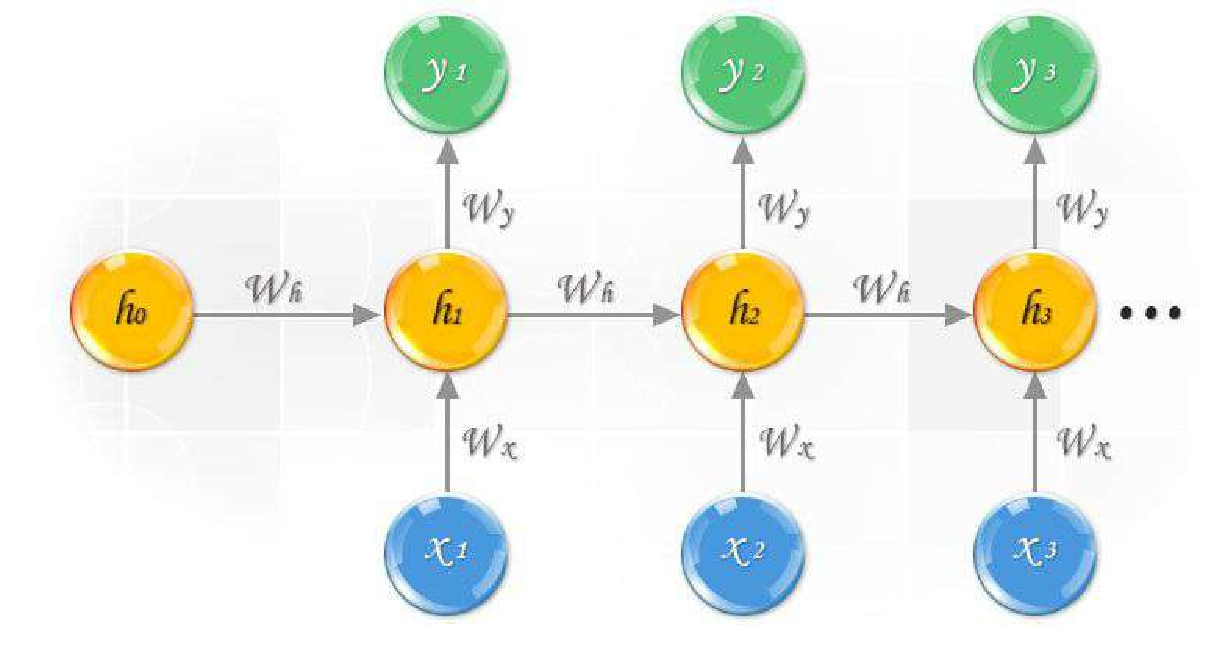
\includegraphics[width=0.9\textwidth]{Imagenes/Redes-Neuronales-Recurrentes}
	\caption{Funcionamiento de las redes neuronales recurrentes}
	\label{fig:1}
\end{figure}


% Añadir más cosas de este enlace https://www.iic.uam.es/innovacion/transformers-en-procesamiento-del-lenguaje-natural/

\section{Otros trabajos relacionados}
\subsection{Generación de historias de vida usando técnias de Deep Learning}
En el curso 2021-2022, la compañera María Cristina Alameda Salas, en su trabajo de fin de grado, Generación de historias de vida
usando técnicas de Deep Learning, desarrolló un sistema basados en técnicas
de Deep Learning que de soporte a la generación de historias de vida. Partiendo de unos datos de entrada en forma de datos estructurados de tipo biográfico, ese trabajo permite la construcción de un sistema de generación de lenguaje natural, transformador de los datos de entrada a un escrito fluido y coherente, que abarque la representación de los datos de partida de manera completa, sin incorrecciones y lo más cercana posible a una redacción humana. Nuestro objetivo ahora sería el desarrollo de un programa que interactuara con el usuario y nos permitiera obtener toda esa información bibliográfica que da lugar a las historias de vida. 
\subsection{Celia}
%https://www.ambito.com/tecnologia/asi-es-celia-la-inteligencia-artificial-adultos-mayores-que-puede-detectar-indicios-alzheimer-n5921639
Celia es un chatbot impulsado por inteligencia artificial (IA) desarrollado por la compañía Atlantic, con el respaldo de la Xunta de Galicia en España. Este chatbot tiene como objetivo acompañar, entretener y brindar asistencia a las personas mayores y dependientes, y se destaca por su capacidad para detectar indicios y patrones de enfermedades neurodegenerativas, como el Alzheimer, mediante el análisis de la voz del usuario.

A diferencia de otros asistentes de conversación como Alexa o Siri, Celia va más allá al utilizar herramientas biométricas para medir y monitorear parámetros indicativos no solo de enfermedades neurológicas, sino también de condiciones emocionales como la ansiedad y la depresión.

Celia está disponible para su uso a través de tres plataformas: WhatsApp, la versión web y una aplicación oficial disponible actualmente solo para dispositivos Android. Los usuarios pueden interactuar con Celia a través de mensajes de texto o de voz, y la instalación es sencilla, lo que permite un acceso rápido y eficiente a este recurso tecnológico.

Una característica destacada de Celia es su capacidad para tomar la iniciativa en las conversaciones y proponer actividades sin necesidad de instrucciones. Además, ofrece la posibilidad de establecer recordatorios para citas médicas o la toma de medicamentos, brindando un apoyo integral en la gestión de la salud de los usuarios.